\section{Computational modelling}
\label{chap1:sec:computational_modelling}

The computational modelling is a multidisciplinary field involving physics, mathematics, and computer science, which has enabled overcoming ever-increasing complexity of engineering problems in the last decades.
The general methodology consists in using mathematical models to describe the physical phenomena in engineering problems, which are then solved with the use of proficient numerical methods and advanced computer algorithms.
In that regard, the computational modelling has become a comprehensive and self-contained scientific discipline, which nowadays is subject of extensive research in many fields of natural sciences and engineering.
The computational modelling has known an expanding application in many research fields, as happens in the polymer processing industry, which has been also taking advantage of this powerful tool to overcome the drawbacks of the usual trial-and-error approaches~\cite{chap1:1998lin,chap1:2000nizami,chap1:2003smith,chap1:2004nobrega,chap1:2006nobrega,chap1:2008nobrega,chap1:2014yang,chap1:2016marques,chap1:2017marques1,chap1:2016habla}.
The present section describes the general methodology of computational modelling, whereas the subsequent sections provide relevant information concerning the mathematical models and the numerical methods.

\subsection{General methodology}
\label{chap1:subsec:computational_modelling_general_methodology}

The computational modelling has seen constant development from its inception.
Since then, innovative approaches have continuously emerged to address the needs and limitations of the industry in solving their problems.
The general methodology of the computational modelling is comprehensively described in the book of M. Sch\"afer, 2006~\cite{chap1:2006schafer}.
Additionally, the books of R.R. Huilgol et al., 1997~\cite{chap1:1997huilgol}, R.G. Owens et al., 2002~\cite{chap1:2002owens}, and M.J. Crochet et al., 2012~\cite{chap1:2012crochet}, for instance, provide a particular focus on the computational modelling applied to fluid mechanics and rheology, as applied in polymer processing applications.
A schematic view of the general methodology is illustrated in Figure~\ref{chap1:fig:computational_modelling_computational_modelling_methodology}, which is briefly described hereafter.

\begin{figure}[!htb]
\centering
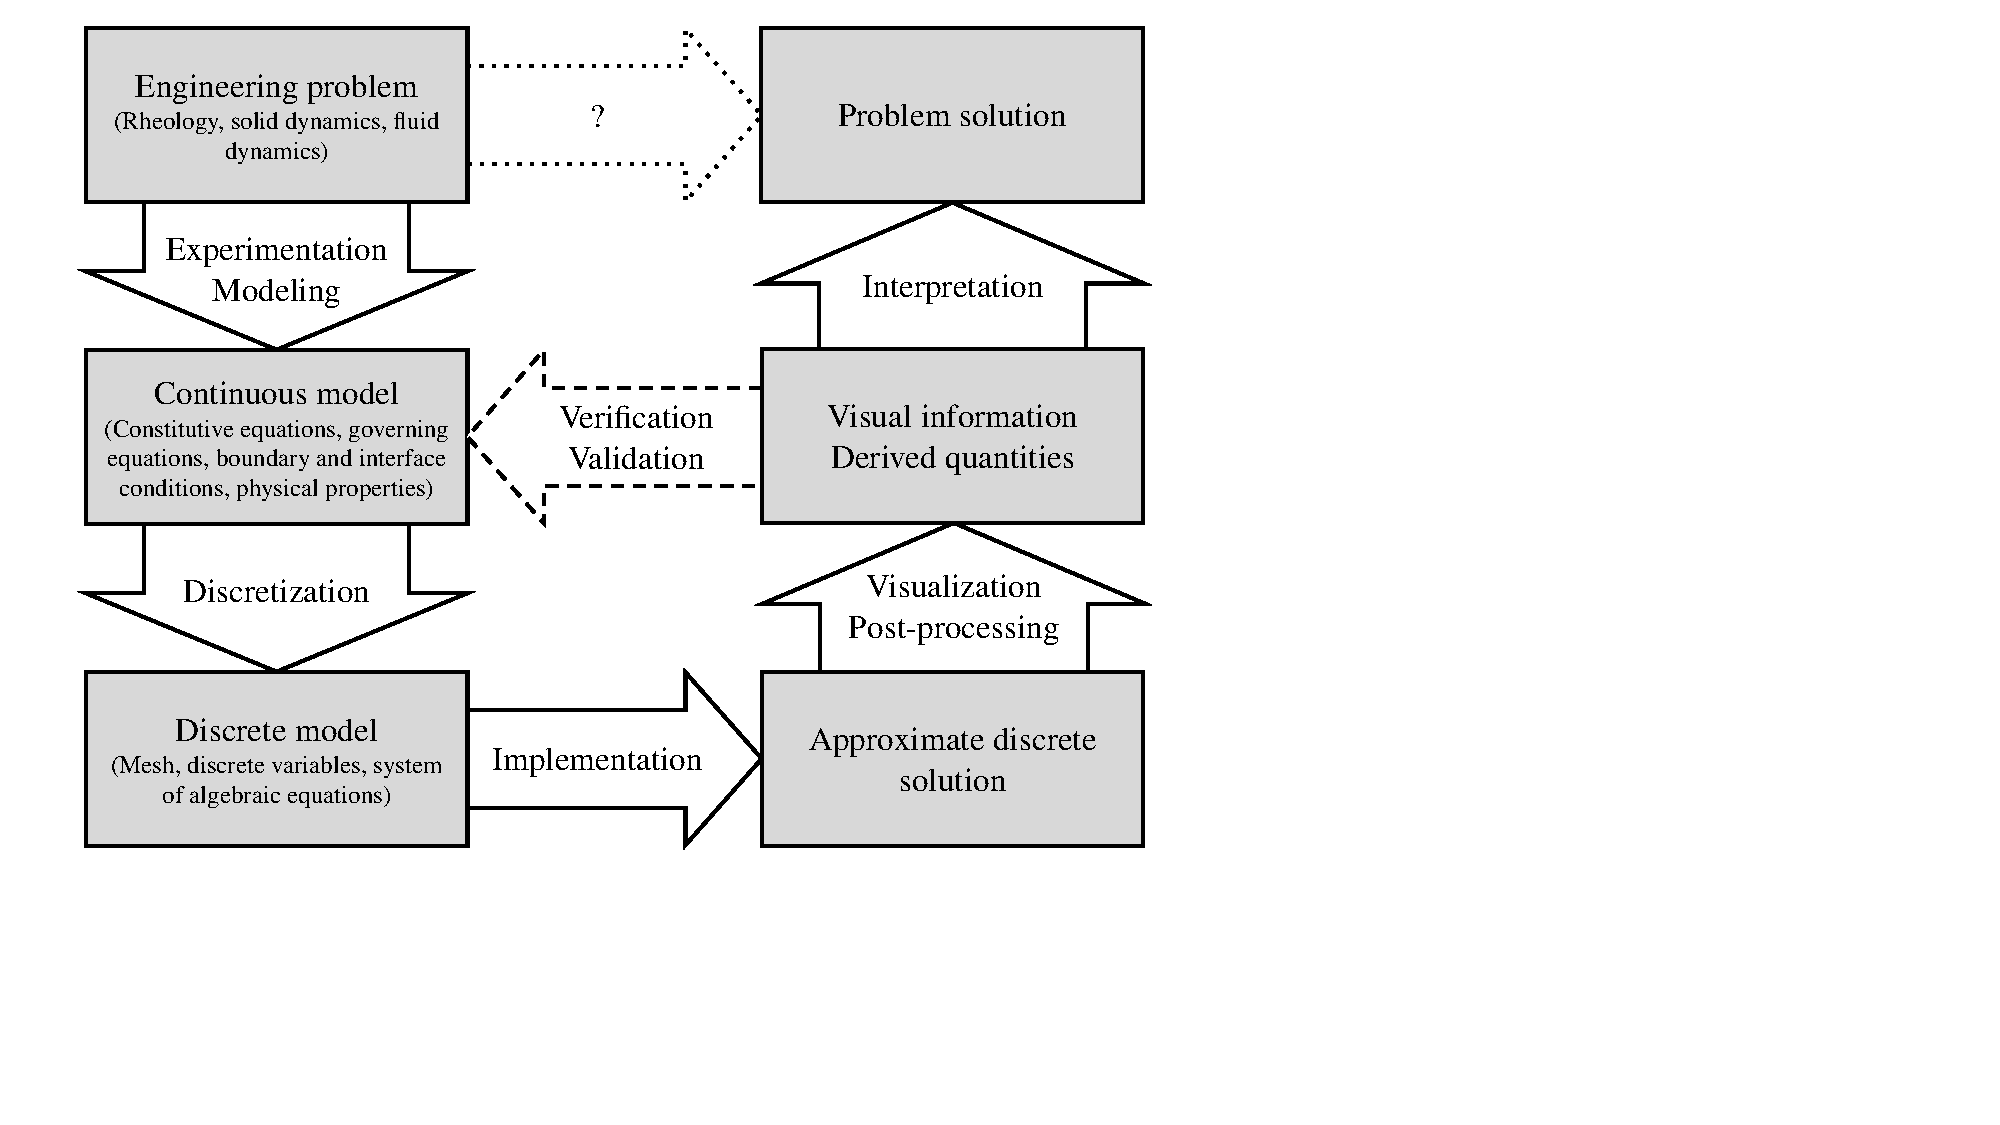
\includegraphics[width=0.75\textwidth]{chap1/include/figures/computational_modelling_methodology.pdf}
\caption[The general methodology of the computational modelling for the solution of engineering problems.]{The general methodology of the computational modelling for the solution of engineering problems (adapted from M. Sch\"afer, Computational engineering: Introduction to numerical methods, Springer, Berlin, 2006).}
\label{chap1:fig:computational_modelling_computational_modelling_methodology}
\end{figure}

The first step consists in defining the geometry and the mathematical models for the physical phenomena involved in the problem of interest.
For instance, constitutive equations derived from rheological principles describe the phenomenological relationships between mechanical variables (and eventually also thermal variables) of fluids in motion.
On the other side, governing equations derived from the solid or fluid mechanics theories model the heat and mass transfer according to the materials physical properties.
Boundary conditions are also required to impose the physically sound limits of the problem unknowns, whereas interface conditions impose the interaction between different materials or regions in contact.
These mathematical models comprise several unknown physical variables, necessary to quantitatively describe the physical phenomena, such as temperature, velocity, stress, and pressure.
Moreover, they were were initially derived from an analytic and experimental process, where conservation Laws or principles were gradually developed and adapted in an attempt to explain the experimental observations.
However, the comprehensive literature available nowadays on mathematical models, also under continuous evolution, allows engineers to adequately describe the physical phenomena in a wide range of problems.
Similarly, the physical properties of the materials are usually determined based on experimentation, for which extensive documentation is also available for most materials~\cite{chap1:2001morrison,chap1:2014beer}.

The mathematical models are often complex, comprising systems of partial differential equations intractable analytically when considering geometries with practical interest (otherwise, the computational modelling methodology would be unnecessary).
In that regard, proficient numerical methods were developed to solve these mathematical models and provide an approximate solution to the associated unknown physical variables.
The usual strategy consists in transforming the continuous model into a discrete model, referred to as discretization, which can be solved using algebra techniques and advanced computer algorithms.
This discretization procedure is performed at two levels, firstly at the level of the problem geometry, and secondly at the level of the mathematical models, as detailed hereafter.

In the first part of the discretization, mesh generation techniques subdivide the geometry into a contiguous mesh of discrete elements, usually consisting of triangles or quadrilaterals (in the two-dimensional case), although any element type can be considered.
Meshes are often classified as structured or unstructured according to the spatial arrangement of the cells, as illustrated in Figure~\ref{chap1:fig:computational_modelling_meshes}.
In structured meshes, the arrangement of the cells is regular, which often leads to more efficient computer memory management and usage, due to the trivial connectivity between neighbour mesh elements.
Moreover, mesh generation algorithms for structured meshes are simple to implement and computationally efficient, although they become cumbersome, or impossible, to adapt and apply in complex geometries, as those arising in typical engineering problems.
In contrast, unstructured meshes have an irregular arrangement of the cells, which makes the mesh generation simpler to adapt to complex geometries.
However, more elaborated algorithms must be implemented, often leading to more computationally expensive memory management and usage, and there is a wide range of open-source software available for mesh generation purposes.
Another advantage of unstructured meshes is the greater ease of creating local refinements, often demanded to increase the accuracy of the solution in critical (large gradient) regions.

The second part of the discretization concerns the partial differential equations in the mathematical models and the associated physical variables defined for the whole problem geometry.
One common approach is to represent the physical variables in the continuous problem as piece-wise numerical variables, usually associated to the cells or the vertices, or even both, depending on the technique.
These variables correspond to unknowns of the discrete model, which is derived from a discretization method used to provide algebraic approximations to the partial differential equations in each reference mesh element, usually the cells or the vertices.
In that regard, a linearization process is usually necessary in the case of non-linear models before the discretization method is applied.
The algebraic equations composing the discrete model can be understood as local representations of the physical phenomena, being more meaningful or more abstract according to the discretization method.
In any case, each equation relates linearly a set of discrete variables in the vicinity of the reference mesh element, which ultimately connects all the equations due to common discrete variables.
There are many discretization methods, where the choice depends on many factors, such as the partial differential equations, the type and arrangement of the mesh elements, or the numerical properties of the method.
For instance, some discretization methods can take advantage of orthogonal structured meshes, that is, when the cell vertices are aligned in orthogonal coordinates, leading to more straightforward derivations and more computationally efficient simulations.
Finally, regardless of the discretization method, the discrete model usually consists of a large number of algebraic equations for the discrete variables, which are then assembled in a system of linear equations.

\begin{figure}[!htb]
\centering
\begin{tabular}{@{}c@{\hskip 0.5cm}c@{\hskip 0.5cm}c@{}}
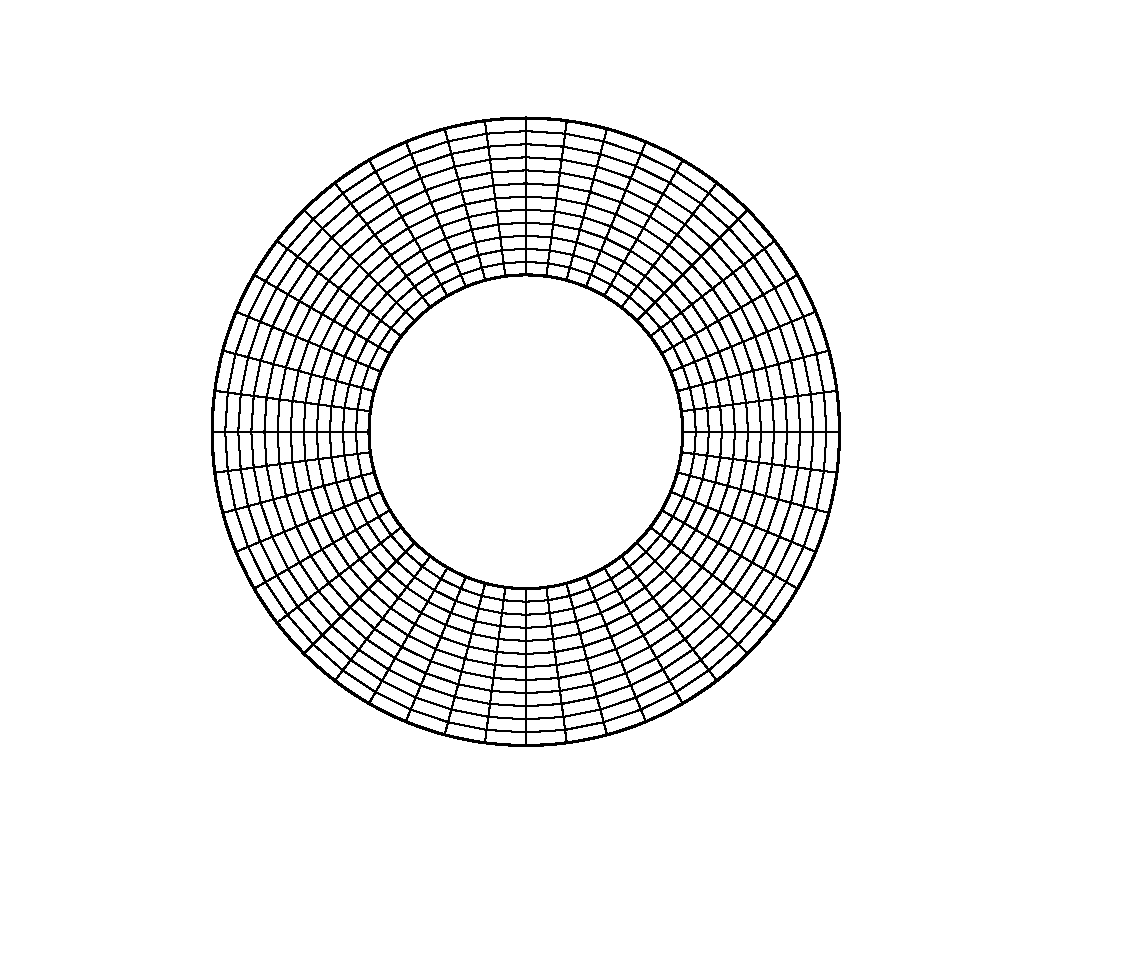
\includegraphics[width=0.3\textwidth]{chap1/include/figures/structured_mesh.pdf}
& 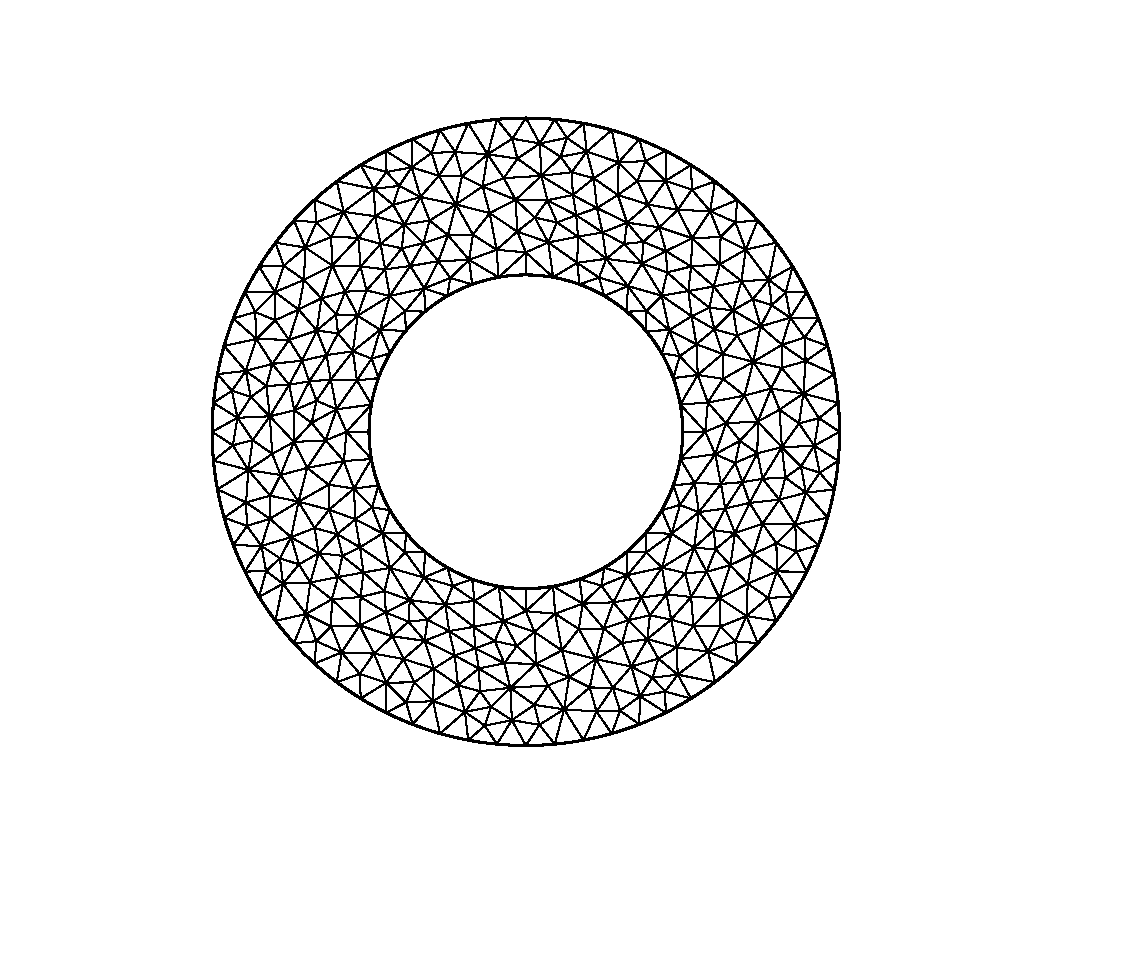
\includegraphics[width=0.3\textwidth]{chap1/include/figures/unstructured_mesh.pdf}
& 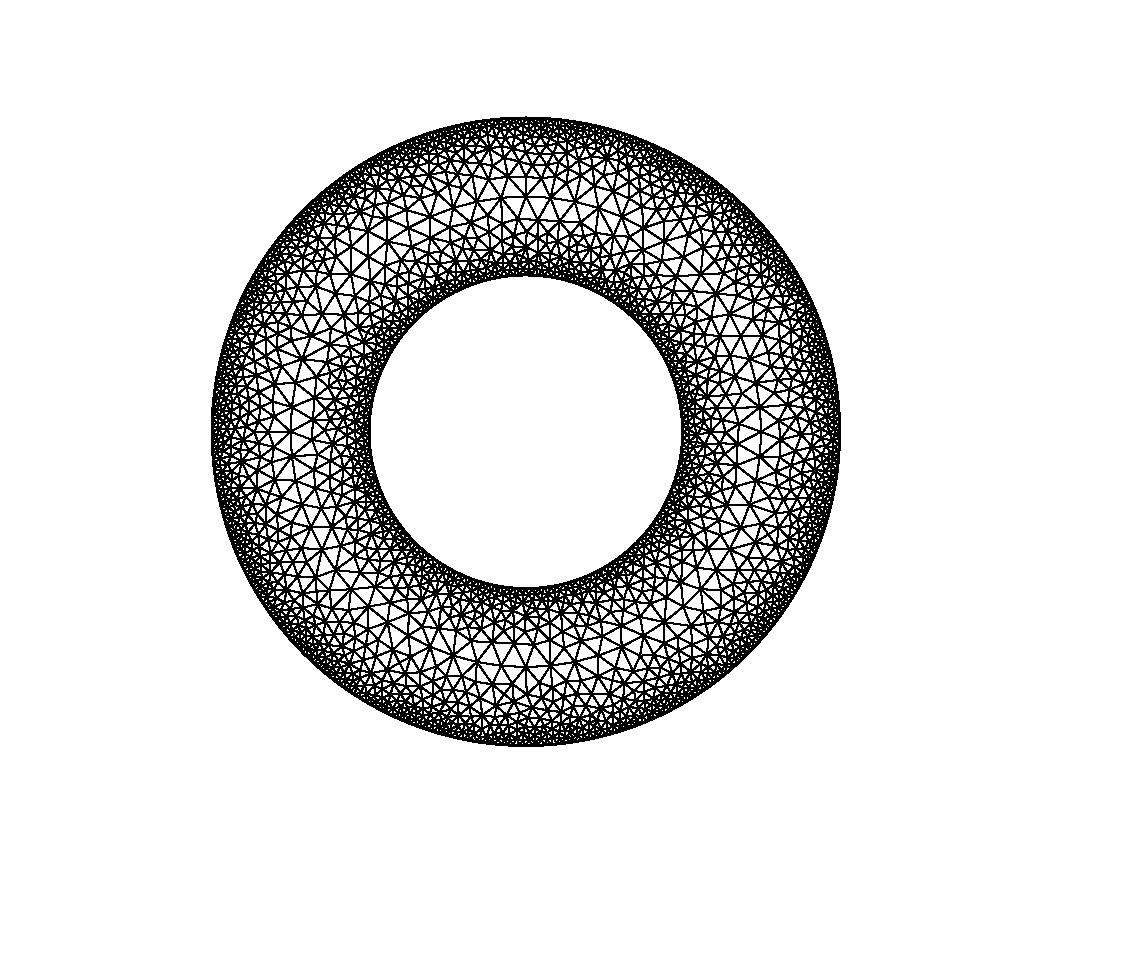
\includegraphics[width=0.3\textwidth]{chap1/include/figures/locally_refined_mesh.pdf}\\
\small(a) Structured quadrilateral & \small (b) Unstructured triangular & \small (c) Refined unstructured\\
\small mesh. & \small mesh. & \small mesh.
\end{tabular}
\caption{Types of meshes for an annular domain.}
\label{chap1:fig:computational_modelling_meshes}
\end{figure}

The system of linear equations is solved with matrix algebra techniques, which provides an approximate solution of the physical variables in the continuous problem in terms of numerical variables.
In practical problems, meshes consisting of thousands or even hundreds of millions of elements are used to provide enough accuracy and, therefore, a large number of numerical variables are computed in the discrete model.
In that regard, the computational aspects become much more relevant, and the implementation with advanced computer algorithms is crucial in the quest for efficient simulations, whose results are obtained in a reasonable time frame.
The approximate solution is not intuitively understood by looking at such a large number of variables, consequently suitable visualization software with post-processing capabilities is used to provide visual information and derive other physical quantities.
Finally, the data is interpreted in the context of the problem, providing means of evaluating and addressing the shortcomings of the application, for instance, to improve the process efficiency.

\subsection{Validation and verification}
\label{chap1:subsec:computational_modelling_validation_and_verification}

The application of the computational modelling allows obtaining an approximate solution for the problem, which is, therefore, prone to errors that should be investigated in the quest for a reliable methodology.
In that regard, the validation of the methodology inspects the quality of the mathematical models in describing the physical phenomena, whereas the verification concerns the quality of numerical methods in solving the mathematical models.
Besides the modelling error, two primary numerical sources are contributing to the error of the approximate solution, as illustrated in Figure~\ref{chap1:fig:computational_modelling_computational_error}.
The first error source is the discretization of the continuous model, which results in a system of linear equations that approximates the partial differential equations locally in the mesh elements.
Therefore, assuming that the solution of the continuous model can be determined analytically, and the solution of the system of linear equations is computed exactly, there would be still a discretization error.
In that case, the accuracy strongly depends on the mesh and the discretization method.
On the other side, the solution of the system of linear equations cannot be computed exactly due to the truncated representation of real numbers in computers, which is also a source of rounding errors.
Moreover, iterative matrix algebra techniques are often used to accelerate the computation process, for which the solution is usually computed, satisfying a residual tolerance.
Indeed, the total numerical error is a combination of the discretization error and the computation error.

The common practice of verification consists in using specific techniques to assess the behaviour of the numerical method, namely in terms of consistency, accuracy, convergence, robustness, and stability.
Analytical techniques are ideally employed to derive or estimate these properties, whereas such approach becomes cumbersome, or even infeasible, for some numerical methods due to its characteristics.
In that regard, numerical benchmarks are usually employed, where several test cases are manufactured with specific difficulties to check the capabilities of the numerical method.
Consistency, accuracy, convergence, robustness, and stability are then evaluated through some kind of error inspection of the approximate solution under mesh refinement.
After checking that the numerical method is capable of solving the model appropriately, the validation phase usually consists in comparing the approximate solution with experimental measurements.
In that regard, the mathematical models are questioned and revised accordingly, often choosing different constitutive or governing equations or even determining the response of the physical properties under different situations.

\begin{figure}[!htb]
\centering
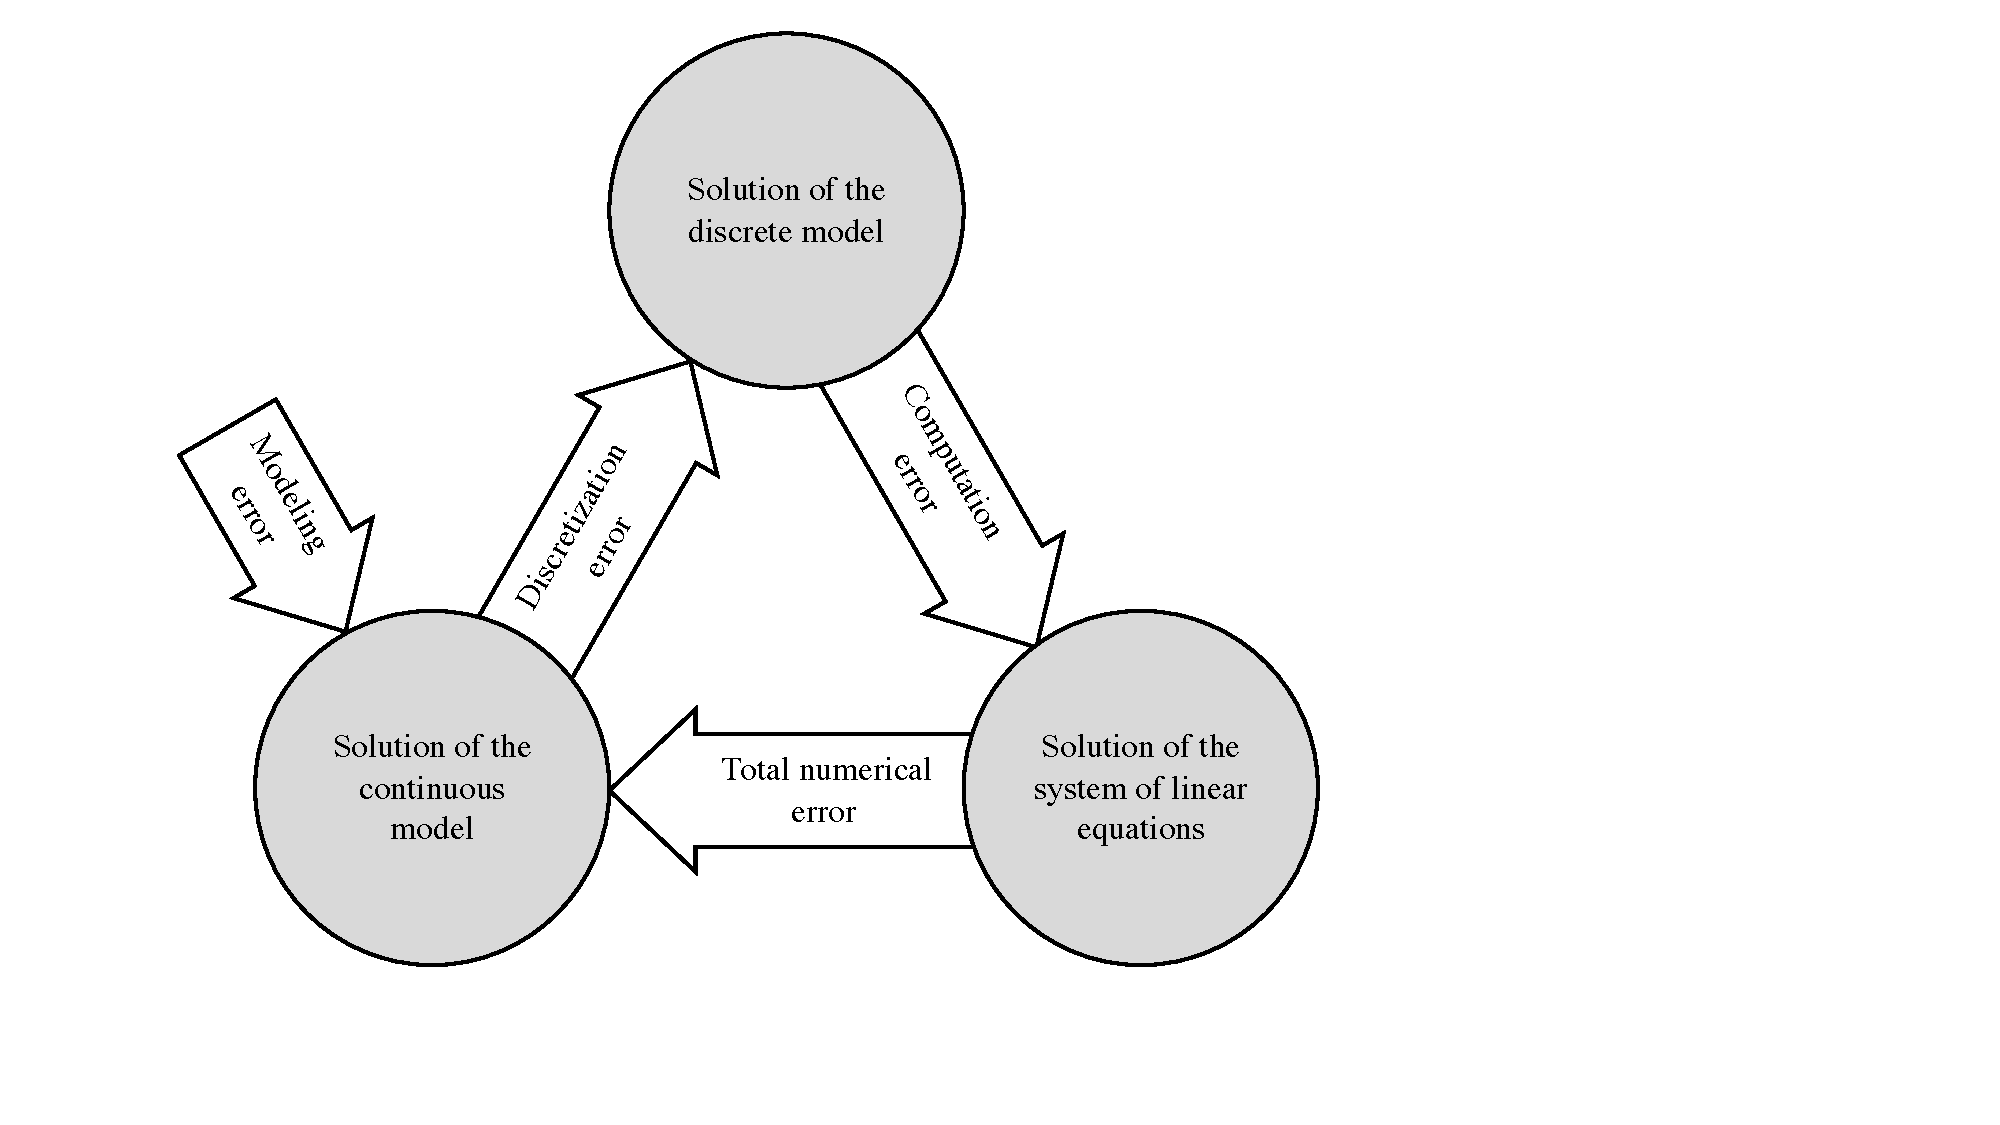
\includegraphics[width=0.75\textwidth]{chap1/include/figures/computational_modelling_error.pdf}
\caption[Numerical errors of the computational modelling for the solution of engineering problems.]{The general methodology of the computational modelling for the solution of engineering problems (adapted from M. Sch\"afer, Computational engineering: Introduction to numerical methods, Springer, Berlin, 2006).}
\label{chap1:fig:computational_modelling_computational_error}
\end{figure}

\subsection{Advantages and limitations}
\label{chap1:subsec:computational_modelling_advantages_and_limitations}

The computational modelling has become a fundamental instrument in many research fields, which includes the polymer processing industry.
Indeed, the benefits of using the computational modelling approach to complement the common trial-and-error experimental based approaches are remarkable.
Firstly, several scenarios of system geometries, processing conditions, cooling conditions, physical properties, among others, can be virtually investigated in the quest of an optimal processing configuration and operation.
Consequently, it reduces the amount of material, time, and money usually required in trial-and-error experimental based approaches, whereas the use of nowadays powerful computers allows finding more efficiently the optimal processing configuration.
Another advantage of the computational modelling approach is the possibility to assess virtually the physical variables at any location, including those that are usually inaccessible through experimentation.
Moreover, it often gives a more comprehensive insight into the physical phenomena due to the simultaneous assessment of several physical variables and derived quantities relevant to the problem.
Despite these benefits, experimental measurements are always required to validate both the mathematical models and the computed results.
In that regard, the development of experimental techniques is an ideal and necessary complement for the practical applicability and utility of the computational modelling approach in the industry.

% end of file
